\documentclass{acm_proc_article-sp}

\usepackage{graphicx}% Include figure files
\usepackage{dcolumn}% Align table columns on decimal point
\usepackage{bm}% bold math
\usepackage{float}
\usepackage{array}
\usepackage{verbatim}
\usepackage{hyperref}% add hypertext capabilities
%\usepackage[mathlines]{lineno}% Enable numbering of text and display math
%\linenumbers\relax % Commence numbering lines

\usepackage{listings}
\usepackage{footnote}
\makesavenoteenv{table}
\makesavenoteenv{table*}
\makesavenoteenv{tabular}

\begin{document}

\title{Self organizing systems WS14 - Exercise 1\\
       Prisoners dilemma}% Force line breaks with \\

\numberofauthors{2}
\author{
\alignauthor
Dragan Avramovski\\
       \email{e1426093@student.tuwien.ac.at}
\alignauthor
Richard Plangger\\
 \email{e1025637@student.tuwien.ac.at}
}

\date{\today}

\maketitle

\begin{abstract}
 The purpose of this assignment is to show the strengths of Multi-Agent systems using the an agent platform. The Prisoners Dilemma problem is implemented with three independent agents that interact. Various agent behaviors are designed to mimic actions of a real human. A more complex is implemented using Bayes' Theorem. Some behavior combinations 
 are used to run an iterative game. The outcomes of these rounds reveal that although the problem seems very simple, it is very hard to trick the opponent agent in the game. Our
 implementation does not implement a very complex communication structure, but it
 was a good opportunity to learn the paradigm and see how communication patterns in
 these system can be built.
\end{abstract}

\keywords{Self organizing systems, Agent, Agent Platform}

%\tableofcontents

\section{Problem Description}
\label{sec:problem-desc}

The Prisoners' Dilemma problem was chosen and implemented in JADE\footnote{\url{http://jade.tilab.com/} Last accessed 11.12.2014}. In this problem, two criminals are convicted for a crime but still not sentenced as there is not enough evidence. Both criminals are interrogated individually and are aware of the consequences. The greatest challenge they face is what action to take. Depending on their decision it is judged how many
years each of them should spent in jail. 
The possible outcome matrix of the problem is shown with Table 1 and it contains all the possible years for a prisoner of the game in respect to the chosen actions.

\begin{table}
\centering
\begin{tabular}{l | l | l}
                     & $P_1$ accuses    & $P_1$ stays silent\\
  \hline
  $P_2$ accuses      & $P_1: 2, P_2: 2$ & $P_1: 3, P_2: 0$ \\
  \hline
  $P_2$ stays silent & $P_1: 0, P_3: 2$ & $P_1: 1, P_2: 1$ \\
\end{tabular}
\caption{Prisoners' Dilemma. Sentences in years depending on the decision of the each prisoner}
\label{tab:prisoner-opt}
\end{table}

There are two actions available: Accuse or Stay Silent and these actions define the possible outcome matrix shown in Table~\ref{tab:prisoner-opt}. The possible outcomes reveal two main concepts: Rational and Irrational.
Being rational means choosing the dominant strategy which is to play Accuse. It is dominant as only by playing rational a prisoner could get away with nothing. If they both play their dominant strategies the game ends up in equilibrium ($P_1$=2 and $P_2$=2). 
Being irrational means they always loose but it could lead them to the optimum result for both, which is to stay silent ($P_1$=1 and $P_2$=1). This strategy is a high risk for both of them as they could end up with maximum sentence. There are three agents implemented: Judge and two prisoners. The Judge agent is a very basic one and is implemented with a static behavior. The judge announces the sentence 
to each prisoner individually after both have told them their action.
The behavior of the prisoner agents is implemented with different strategies:

\begin{enumerate}
   \item Random. The prisoner decides using a random generator.
   \item Static. The prisoner decides his action depending on his starting value.
   \item Titfortat. This behavior only considered the last decision of the judge. It replays
      the action of the other prisoner. Initially the prisoner plays silent to start the first
      round.
   \item Aggressive. This behavior tries to trick the other prisoner. Initially this
      behavior plays accuse. It tracks a window of the last $x$ rounds and sums up
      the years it got for it. Having this value below a certain threshold $y$ it stays aggressive.
      Depending on the initial configuration it plays another behavior if the threshold
      is exceeded.
   \item Optimistic. The prisoner forgives and has a tendency to cooperate. If it finds out
      that his optimistic behavior is abused, he changes into aggressive mode.
   \item Bayes. A learning Agent implemented with conditional probability - Bayes' Theorem~\cite{gupta2011introduction}.
		The agent trains a model using previous rounds and plays a certain strategy. After his model has been trained he computes the probabilities and tries to take advantage of his knowledge.
\end{enumerate}

\section{Learning Agent - Bayes}
As we put the most effort into this behavior, this section is dedicated to the ``learning'' agent.
In the following examples $P_2$ learns and tries to predict the next actions of $P_1$. The requirement is implemented by using conditional Probability - Bayes Rule.
\[
    P(\textbf{C}|\textbf{x}) = P(\textbf{x}|\textbf{C}) \frac{P(\textbf{C})}{P(\textbf{x})}
\]

$C$ is the class/action to be predicted. Either Accuse or Silent for $P_1$.
$x$ is the rounds the algorithm has seen so far. Accuse or Silent from $P_2$.


\subsection{Example:}
Q: What is the probability of $P_1$ playing $Silent$ given that $P_2$ played $Accuse$? 
\begin{center} 
P($P_1$:$Silent$$|$$P_2$:$Accuse$)=?
\end{center}

The class $C$ = $Silent$ given the predictor data $x$ = $Accuse$. 
This question can only be answered using prior knowledge given in the data set in Table~\ref{tab:training-set}.

\begin{table}
\centering
\begin{tabular}{l | l }
 $P_1$ decisions & $P_2$ decisions \\
  \hline
$Accuse$&$Silent$\\
  \hline
$Accuse$&$Silent$\\
  \hline
$Accuse$&$Accuse$\\
  \hline
$Accuse$&$Accuse$\\
  \hline
$Accuse$&$Accuse$\\
  \hline
$Accuse$&$Accuse$\\
\hline
$Silent$&$Accuse$\\
\hline
$Silent$&$Silent$\\
\hline
$Silent$&$Silent$\\
\end{tabular}
\caption{Sample training set}
\label{tab:training-set}
\end{table}

To extract frequency and likelihood information the knowledge from the
last rounds is counted and summed up in Table~\ref{tab:frequency-val}.

\begin{table}
\centering
\begin{tabular}{l | c | c}
                     & $P_1$ accuses    & $P_1$ stays silent \\
  \hline
  $P_2$ accuses      & 4 				& 2 				 \\
  \hline
  $P_2$ stays silent & 1 				& 2   				 \\
\end{tabular}
\caption{Frequency Values based on the Training set in Table~\ref{tab:training-set}}
\label{tab:frequency-val}
\end{table}

\begin{table*}
\centering
\begin{tabular}{l | c | c | l}
                     & $P_1$ accuses       & $P_1$ stays silent  & $P(x)$ \\
  \hline
  $P_2$ accuses      & 4/5   	 & 2/4	   &  P($P_2$:$Accuse$)=6/9 	  \\
  \hline
  $P_2$ stays silent & 1/5		 & 2/4 	   &  P($P_2$:$Silent$)=3/9 	  \\
  \hline
  $P(C)$ 			 & P($P_1$:$Accuse$)=5/9 & P($P_1$:$Silent$)=4/9 &    \\
  \end{tabular}
\caption{Likelihood Values based on the Training set in Table~\ref{tab:training-set}}
\label{tab:likelihood-val}
\end{table*}

Then by following the Bayes algorithm the likely hood must be calculated. The results
are shown in Table~\ref{tab:likelihood-val}.

Q: What is the probability of $P_1$ playing $Silent$ given that $P_2$ played $Accuse$? 
\begin{center} 
P($P_1$:$Silent$$|$$P_2$:$Accuse$)=0.3333
\end{center}

Q: What is the probability of $P_1$ playing $Accuse$ given that $P_2$ played $Accuse$? 
\begin{center} 
P($P_1$:$Accuse$$|$$P_2$:$Accuse$)=0.6666
\end{center}

\begin{comment}
% Two examples are enough to get a feeling I think!
Q: What is the probability of $P_1$ playing $Accuse$ given that $P_2$ played $Silent$? 
\begin{center} 
P($P_1$:$Accuse$$|$$P_2$:$Silent$)=0.3333
\end{center}

Q: What is the probability of $P_1$ playing $Silent$ given that $P_2$ played $Silent$? 
\begin{center} 
P($P_1$:$Silent$$|$$P_2$:$Silent$)=0.6666
\end{center}
\end{comment}

\section{Implementation and Setup}

Our implementation uses the JADE agent framework. We use gradle as a build and dependency management tool, but we also provide a simple packaged jar. There are three actors
involved on an actor platform. The judge $J$ is the communication partner for both
prisoners ($P_1$,$P_2$). Both prisoners are not allowed to communicate and only
send their messages to the judge.

The behavior of $J$ is static and implements the logic we explained earlier. It can be
found in the class JudgeBehaviour. It is cyclic (never ending until manual intervention) and awaits two messages from different prisoners and sends back the sentence.

\begin{lstlisting}
$ java -cp libs/jade.jar:libs/dilemma.jar \
    jade.Boot -name dilemma -gui \
    -agents judge:sos.agent.Judge
\end{lstlisting}

The previous command starts the agent and registers the judge Agent to the dilemma platform.
$J$ is the central role, thus it provides the gui to observe the platform.

The prisoners are started in a similar way:

\begin{lstlisting}
$ java -cp libs/jade.jar:libs/dilemma.jar \
    jade.Boot -container -agents \
    p1:sos.agent.Prisoner(static,accuse) \
    -Drounds=20
\end{lstlisting}

This starts a prisoner named p1 and plays a static behavior sending accuse for 20 rounds.
A full list of all possible combinations can be retrieved by removing the parameters for
the prisoner. Note that for the platform to work you need to start two prisoners
with the name p1 and p2. After a prisoner has completed his rounds he will print
the stats of his iteration including the stats of the other prisoner.

\subsection{Communication}

While familiarizing with the JADE platform we learned that we basically have several options
on how to let the agents communicate.

\begin{itemize}
	\item Let the judge provide a service (register on the platforms yellow pages) and let
    the prisoners lookup the service and use it
    \item Judge and prisoners have unique names. This allows to directly address the other
    agents.
    \item Send messages into the platform and flag them with certain properties (e.g. Ontology: Prisoner Dilemma) and let all participants filter the messages.
\end{itemize}

While all of them have their strengths and weaknesses we decided to directly address the agents.
The motivation of this was mostly because in real life this works quite the same. You
know which court you must go to to pledge innocent and receive your sentence. This allowed
us to filter the messages in the behavior using the AID. The behavior of sending their
decision and receiving the sentence for every prisoner is the same,
thus we abstracted this behavior into the base class sos.agent.behaviour.BasePrisonerBehaviour.

The programming style of receiving messages in JADE is not very intuitive at first glance.
We would have expected blocking behavior for receiving messages, but one must either
poll for the message (bad performance) or change the control flow and call \lstinline!block()! 
and return the action method. Rethinking this our conclusion is that it resembles behavior in the real world. If you send out a message and want your answer back, the answer often is
asynchronous. In a restaurant whenever you order a dish, you could constantly poll the waiter if it is ready. But this does not make sense and would drive the waiter crazy. The normal
behavior would be to wait until you receive a new message (your dish arrives) and then process it (eat it).

\begin{figure*}
\begin{center}
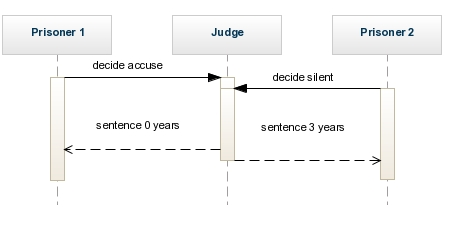
\includegraphics{dilemma-sequence}
\end{center}
\caption{Sequence diagram of one round of communication}
\label{fig:dilemma-sequence}
\end{figure*}

Figure~\ref{fig:dilemma-sequence} shows a communication round as a UML sequence diagram.
One round is illustrated. The judge awaits two decisions (accuse|silent) from two different
prisoners. He then later replies with the sentence.

\begin{figure*}
\begin{center}
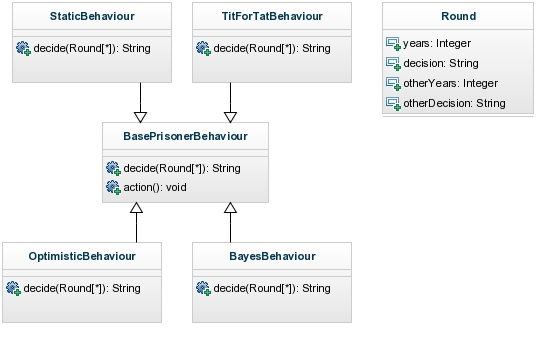
\includegraphics{dilemma-minimal-classes}
\end{center}
\caption{Subset of the classes as UML class diagram}
\label{fig:dilemma-classes}
\end{figure*}

Figure~\ref{fig:dilemma-classes} show a subset of the classes that we have implemented.\footnote{Parameter for the function decide is a list of rounds (written as Round[*]).}
Our base prisoner behavior implements the \lstinline!action()! method to communicate with
the judge. The selected behavior (depending on the start parameter of the agent) then
gets the list of previous rounds. This is the knowledge he operates on. In the
different behaviors we have used this information to try to implement rational agents,
irrational agents.

\section{Testing our implementation}

After presenting your implementation we would like to examine the agents and their behaviors.
In the following we will evaluate some behavior combinations running the prisoners for 100 rounds.
The most interesting property is the sum of years, and the sum of years for each specific prisoner.

Here is a list of certain combination we believe that are interesting.

\begin{enumerate}
	\item $P_1$ random, $P_2$ Titfortat. Since Titfortat replays the last round, and the
    other prisoner plays random, $P_2$ should have nearly equal years than $P_1$.
    \label{item:p1random-p2titfortat}
    
	\item $P_1$ optimistic, $P_2$ aggressive. The aggressive prisoner tries to gain the
      most out of the optimistic behavior. We suspect that the aggressive might have a slight advantage, because he can trick the optimistic prisoner for some rounds.
    \item $P_1$ bayes, $P_2$ random. $P_1$ after having seen 20 rounds, should keep a window of 20 rounds that he uses to predict the other action. Here we also expect that bayes should have a slight advantage, but should not be worse than $P_2$.
    \item $P_1$ bayes, $P_2$ optimistic. Similar to the previous point, bayes should train
    a model, that predicts the optimistic behavior. We expect the two to minimize the years (after the initial random phase has worn out).
    \item $P_1$ bayes, $P_2$ aggressive. $P_1$ should learn the aggressive behavior and also
    play aggressive until the end.
    \item $P_1$ bayes, $P_2$ titfortat. We think that in this behavior it greatly depends
    on the initial model how bayes behaves.
\end{enumerate}

\begin{table*}
\centering
\begin{tabular}{ l | c | c | c }
Modus & $P_1$ years & $P_2$ years & Sum years \\
\hline
1. $P_1$ random, $P_2$ titfortat & 
   $(147)_1$,$(140)_2$,$(148)_3$ &
   $(147)_1$,$(143)_2$,$(142)_3$ &
   $(294)_1$,$(283)_2$,$(290)_3$ \\
\hline
2. $P_1$ bayes, $P_2$ titfortat\footnote{$P_1$ uses 20 rounds to train and maintain his model} & 
   $(182)_1$,$(187)_2$,$(111)_3$ &
   $(188)_1$,$(184)_2$,$(111)_3$ &
   $(370)_1$,$(371)_2$,$(222)_3$ \\
   
\hline
3. $P_1$ optimistic, $P_2$ aggressive\footnote{
Parameters for $P_1$ are trust level = 10, $P_2$ plays static silent when years are above the threshold. In round 1, window = 10, threshold = 0.6, round 2: window = 20, threshold = 0.6,
round 3: window = 20, threshold = 0.5
} & 
   $(177)_1$,$(182)_2$,$(183)_3$ &
   $(141)_1$,$(140)_2$,$(120)_3$ &
   $(318)_1$,$(322)_2$,$(303)_3$ \\
\hline
4. $P_1$ bayes, $P_2$ random\footnote{$P_1$ uses sliding window of 10 rounds to train and maintain his model} & 
   $(120)_1$,$(108)_2$,$(135)_3$ &
   $(204)_1$,$(222)_2$,$(162)_3$ &
   $(324)_1$,$(330)_2$,$(297)_3$ \\
   
\hline
5. $P_1$ bayes, $P_2$ optimistic\footnote{$P_2$ has a trust level = 10, $P_1$ uses sliding window of 20 rounds to train and maintain his model} & 
   $(155)_1$,$(150)_2$,$(154)_3$ &
   $(203)_1$,$(207)_2$,$(205)_3$ &
   $(358)_1$,$(357)_2$,$(359)_3$ \\
   
\hline
6. $P_1$ bayes, $P_2$ aggressive\footnote{Both consider only the last 20 rounds, $P_2$ uses a threshold of 0.6 and plays static silent if he exceeds the threshold, $P_1$ uses 20 rounds to train and maintain his model} & 
   $(194)_1$,$(211)_2$,$(198)_3$ &
   $(140)_1$,$(142)_2$,$(150)_3$ &
   $(334)_1$,$(353)_2$,$(348)_3$ \\
   
\end{tabular}
\caption{Testing the different combinations using our system. Iteration count is always 100. Bayes behavior uses random decisions until he is has enough data (20 rounds)}
\label{tab:tests}
\end{table*}

Table~\ref{tab:tests} show the results of our test cases. The numbers written in subscript on each year denote the round. $(111)_2$ means 111 years on the second test run.

As we have expected for (1.) the years for both prisoners are as if both played random. They
have nearly the same amount of years after 100 rounds. In (2.) we observe the same behavior. But (2.) also depends on the initial model. Since $P_1$ plays random for the first 20 rounds
it determines the model. In round 3 random yielded silent very often which drove the model
of bayes into a state where it predicted that silent is the best choice.

In the third combination (3.) the optimistic agent clearly lost. In each test run he got at least 30 years more than the aggressive one. It mostly depends on the parameter settings for both how bad/good the optimistic agent behaves. But we believe that the optimistic strategy is
quite good, because he only allows the other prisoner to betray him until his trust level falls below zero. After that trust has to be gained again.

Test variation (4.) is very interesting. We expected $P_1$ to have a slight advantage. In fact
he won every round with a mean value of 75 years less. For the
random implementation we used the SecureRandom class to get better random numbers. We
do not know the cause of this. Our best guess is that the sliding window of Bayes helps
him to keep an up to date model and that the random class is not that random at all.

Similar to (3.), in test variation (5.) the optimistic agent loses. 
Here he even gains more years (around 50) than in (3.)
The prediction is really good and keeps $P_1$ from gaining years
when the trust level of $P_2$ drops below zero.

The last test variation (6.) is the only that has beaten the Bayes prediction. An aggressive
agent $P_2$ disguises himself as silent prisoner after he has earned played aggressive.
In the second phase $P_1$ predicts $P_2$ to stay silent (he did so in the last rounds) 
$P_2$ will drop into aggressive behavior again.

\section{Conclusion}

In this assignment we have implemented a simple agent system where two prisoners are able to
cooperate and/or compete against each other. The JADE interface to implement an agent
is simple and stable. It would be interesting to evaluate the platform in more detail
and see more complex communication patterns that are possibly split amongst sever computing nodes.
In addition to that we have implemented several behaviors and let them compete against each other. Some results surprised us. It seems to be a very easily understandable problem, but
in out opinion it is not so easy to trick other agents.
The self organizing aspect of each agent is also very interesting. Because the interface
is very simple you need to communicate to acquire more information. An agent alone can do
very little things, but his capabilities increase tremendously when he gets new information.

\bibliography{ref}
\bibliographystyle{plain}

\end{document}
%
% ****** End of file apssamp.tex ******
